% =====================================================================
%  Report - Project 1: DDS on FPGA (Red Pitaya)
%  Build (from the rapport/ folder):
%     pdflatex rapport.tex && pdflatex rapport.tex
%  (2 passes for the table of contents and references)
% =====================================================================
\documentclass[11pt,a4paper]{article}

% ---------- Language / encoding ----------
\usepackage[T1]{fontenc}
\usepackage[utf8]{inputenc}
\usepackage{lmodern}
\usepackage[english]{babel}

% ---------- Layout ----------
\usepackage[margin=2.2cm]{geometry}
\usepackage{fancyhdr}
\usepackage{graphicx}
\usepackage{float}
\usepackage{subcaption}
\usepackage{booktabs}
\usepackage{amsmath}
\usepackage[per-mode=symbol]{siunitx}
\sisetup{retain-explicit-plus}
\usepackage{xcolor}
\usepackage{tikz}
\usetikzlibrary{arrows.meta,positioning}
\usepackage{listings}
\usepackage[hidelinks]{hyperref}

\graphicspath{{figures/}}
\setlength{\emergencystretch}{3em}
% Allow line breaks after underscores in long signal names
\let\oldunderscore\_
\renewcommand{\_}{\oldunderscore\allowbreak}

% ---------- Header / footer ----------
\setlength{\headheight}{14pt}
\pagestyle{fancy}
\fancyhf{}
\lhead{FPGA -- Project 1: DDS}
\rhead{ELISE M2}
\cfoot{\thepage}

% ---------- VHDL code style ----------
\definecolor{kw}{RGB}{0,0,160}
\definecolor{cm}{RGB}{0,120,0}
\definecolor{bg}{RGB}{247,247,247}
\lstdefinestyle{vhdl}{
  language=VHDL,
  basicstyle=\ttfamily\footnotesize,
  keywordstyle=\color{kw}\bfseries,
  commentstyle=\color{cm}\itshape,
  backgroundcolor=\color{bg},
  numbers=left, numberstyle=\tiny\color{gray},
  frame=single, breaklines=true, showstringspaces=false,
  tabsize=4, columns=fullflexible, keepspaces=true
}
\lstdefinestyle{sh}{
  basicstyle=\ttfamily\footnotesize, backgroundcolor=\color{bg},
  frame=single, breaklines=true, columns=fullflexible
}
% Allows accented characters in code comments
\lstset{literate={é}{{\'e}}1 {è}{{\`e}}1 {à}{{\`a}}1 {ç}{{\c c}}1 {ê}{{\^e}}1 {ù}{{\`u}}1}

% Inserts a figure if the file exists, otherwise a "to add" placeholder box
% usage: \fig{file_name}{caption}{label}
\newcommand{\fig}[3]{%
  \begin{figure}[H]\centering
    \IfFileExists{figures/#1}
      {\includegraphics[width=0.85\linewidth]{#1}}
      {\fbox{\parbox[c][4cm][c]{0.8\linewidth}{\centering\color{gray}
        Figure to add: \texttt{figures/\detokenize{#1}}}}}
    \caption{#2}\label{#3}
  \end{figure}}

% Marker for text still to write (delete once done)
\newcommand{\todo}[1]{\textcolor{red}{[To write: #1]}}

% =====================================================================
\begin{document}

% ---------------------------- Title page ---------------------------
\begin{titlepage}
  \centering
  {\large Université Marie et Louis Pasteur\par}
  {\large ELISE Master -- 2\textsuperscript{nd} year\par}
  \vspace{3cm}
  {\Huge\bfseries Project 1: DDS\par}
  \vspace{0.5cm}
  {\Large Direct Digital Synthesis on FPGA\\(Red Pitaya, Zynq-7010)\par}
  \vspace{3cm}
  {\large \textbf{Authors:} LAST NAME First name -- LAST NAME First name\par}
  \vspace{0.5cm}
  {\large \textbf{Teacher:} NAME\par}
  \vfill
  {\large Academic year 2026--2027\par}
\end{titlepage}

\tableofcontents
\newpage

% =====================================================================
\section{Introduction}
To understand how a direct digital synthesizer (DDS) works before we drive one
in the third project, we described our own DDS in VHDL and
synthesized it on the FPGA of the Red Pitaya board.

\begin{figure}[H]
\centering
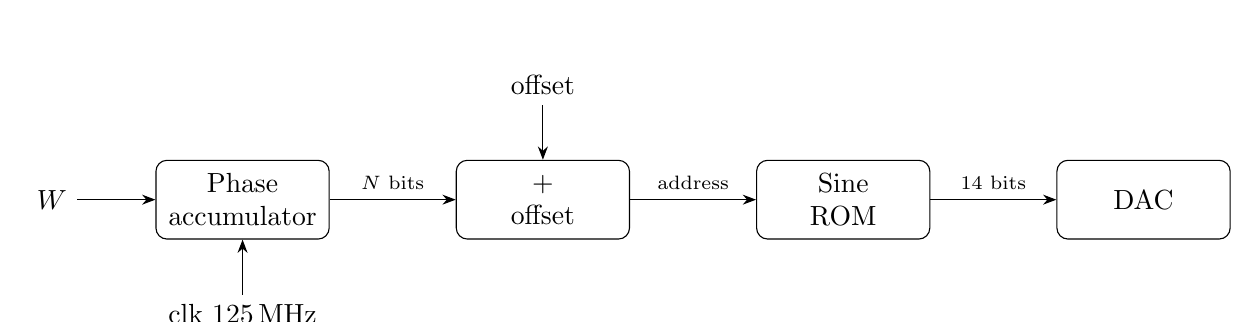
\begin{tikzpicture}[node distance=1.6cm, >=Stealth,
    blk/.style={draw, rounded corners, minimum height=1cm, minimum width=2.2cm, align=center}]
  \node[blk] (acc) {Phase\\accumulator};
  \node[blk, right=of acc] (add) {$+$\\offset};
  \node[blk, right=of add] (rom) {Sine\\ROM};
  \node[blk, right=of rom] (dac) {DAC};
  \draw[->] (acc) -- node[above]{\scriptsize $N$ bits} (add);
  \draw[->] (add) -- node[above]{\scriptsize address} (rom);
  \draw[->] (rom) -- node[above]{\scriptsize 14 bits} (dac);
  \draw[<-] (acc.west) -- ++(-1,0) node[left]{$W$};
  \draw[<-] (add.north) -- ++(0,0.7) node[above]{offset};
  \draw[<-] (acc.south) -- ++(0,-0.7) node[below]{clk \SI{125}{\mega\hertz}};
\end{tikzpicture}
\caption{DDS block diagram}\label{fig:bloc}
\end{figure}

A DDS relies on three blocks (Figure~\ref{fig:bloc}). A phase accumulator, built
as an adder, adds a word $W$ to the current phase on each clock edge. A second adder
then applies a phase offset to this value. Finally, a memory maps each phase to the
amplitude of the desired signal, here a sine wave quantized on 14 unsigned bits.

This principle exploits the linearity of phase. Over a time step $\Delta t$, the phase
of a signal at frequency $f$ increases by $\Delta\varphi = 2\pi f \Delta t$, modulo
$2\pi$. When we encode the phase on $N$ bits, $2^N$ corresponds to $2\pi$, and $W$
becomes the phase increment added at each clock period. The output frequency is then:
\begin{equation}
  f_{out} = f_{clk}\,\frac{W}{2^N}
  \label{eq:fout}
\end{equation}

With the \SI{125}{\mega\hertz} FPGA clock and $N = 10$, we get a frequency step of
$\SI{125}{\mega\hertz}/1024 = \SI{122.07}{\kilo\hertz}$ and a phase resolution of
$\ang{360}/1024 = \ang{0.352}$. Each period of the output signal contains $2^N/W$
samples: as $W$ grows, the output frequency rises and the memory supplies fewer
points per period to rebuild the sine wave.

% =====================================================================
\section{Sine lookup table generation (Octave)}


\begin{equation}
  \mathrm{LUT}(k) = \mathrm{round}\!\left(\frac{\sin(2\pi k/2^N) + 1}{2}\,(2^{14}-1)\right),
  \quad k = 0,\dots,2^N-1
\end{equation}

\lstinputlisting[style=vhdl, language=Octave, caption={Octave script \texttt{sine\_wave.m}}]{../octave/sine_wave.m}

\fig{table_sinus.png}{ROM content: 1024 samples on 14 bits}{fig:lut}

% =====================================================================
\section{VHDL description of the DDS}

\paragraph{Entity interface.} The subject asks for $N$ as a generic, so the entity
declares \texttt{N : integer := 10} before its ports. It has four ports: the clock
\texttt{clk}, the frequency word \texttt{W} and the phase offset
\texttt{phase\_offset} on $N$ bits each, and the 14-bit output \texttt{sine\_out}.
We typed the ports as \texttt{std\_logic\_vector} so the same entity connects
without conversion both to the encapsulating file and to the AXI GPIO outputs in
the Vivado block design. Inside the architecture, we cast them to
\texttt{unsigned} to perform the additions.

\paragraph{Phase accumulator.} A process triggered on the rising edge of
\texttt{clk} adds \texttt{W} to the phase at each cycle:

\begin{lstlisting}[style=vhdl, caption={Phase accumulator}]
-- Phase accumulator
process(clk)
begin
    if rising_edge(clk) then
        phase_acc <= phase_acc + unsigned(W);
    end if;
end process;
\end{lstlisting}

We declared \texttt{phase\_acc} as an $N$-bit \texttt{unsigned}. When the sum
exceeds $2^N-1$, it wraps back to 0 with no extra logic, and this overflow
implements the modulo $2\pi$ of the phase. The design has no reset input:
\texttt{phase\_acc} starts at 0 through its initial value
\texttt{(others => '0')}, which GHDL and the FPGA bitstream both take into
account. The DDS runs continuously and its starting phase does not matter here,
so a reset would add a port without adding a function.

\paragraph{Offset adder.} The ROM address comes from a combinational addition
(Listing~\ref{lst:offset}), which also wraps modulo $2^N$. We placed the offset after the accumulator and not inside it.
Added after, it shifts the phase by a constant and leaves the frequency
unchanged. Added inside the loop, it would accumulate at every clock cycle and
behave like an extra increment of \texttt{W}, changing the output frequency.
\begin{lstlisting}[style=vhdl, caption={Offset adder}, label={lst:offset}]
rom_addr <= phase_acc + unsigned(phase_offset);
\end{lstlisting}

\paragraph{ROM.} We declared the memory as a constant array \texttt{rom\_type} of
1024 entries of type \texttt{integer range 0 to 16383}, filled with the values
from the Octave table described in section~2 (see Appendix~A for the full
listing). Each value goes through \texttt{to\_unsigned(..., 14)} before reaching
the output (Listing~\ref{lst:rom}).
\begin{lstlisting}[style=vhdl, caption={ROM lookup}, label={lst:rom}]
-- ROM Lookup
    process(clk)
    begin
        if rising_edge(clk) then
            -- Convert the integer from ROM back to STD_LOGIC_VECTOR
            sine_out <= std_logic_vector(to_unsigned(SINE_ROM(to_integer(rom_addr)), 14));
        end if;
    end process;
\end{lstlisting}
During synthesis, GHDL (\texttt{ghdl -{}-synth}) recognizes this array as a ROM and
reports \texttt{found ROM "n42", width: 14 bits, depth: 1024}, so the tools map it as
a memory instead of building it from decoding logic. This choice has one limitation:
the array size is fixed at 1024 while $N$ is generic. If we change $N$, we must
regenerate the table in Octave and declare the array as \texttt{0 to 2**N-1}.

\paragraph{Registered output and latency.} We write \texttt{sine\_out} inside a
clocked process, which makes it a register. The DAC then receives stable data,
free of the glitches the combinational adder and ROM produce while settling, and
the path between two registers fits more easily in the \SI{8}{\nano\second}
period of the \SI{125}{\mega\hertz} clock. The cost is latency, which GTKWave
shows: a change of \texttt{phase\_offset} reaches the output after one clock
cycle, since it only crosses the output register, while a change of \texttt{W}
takes two cycles, one to update the accumulator and one to update the output.

% =====================================================================
\section{Simulation (GHDL / GTKWave)}

\subsection{Testbench}
The testbench \texttt{dds\_tb} has no ports. It instantiates the DDS with
\texttt{N => 10}, generates the clock, and applies a sequence of stimuli chosen to
check each property described in section~3. Its signals \texttt{W} and
\texttt{phase\_offset} are declared on 10 bits, so a change of $N$ requires editing
them along with the generic map.

A dedicated process generates the \SI{125}{\mega\hertz} clock with a period of
\SI{8}{\nano\second}. It loops while the boolean \texttt{sim\_end} stays false, and
the stimulus process sets \texttt{sim\_end} to true after the last test. The clock
process then reaches its final \texttt{wait}, no event remains in the simulation,
and GHDL stops on its own without a \texttt{-{}-stop-time} option.

The stimulus process first waits \SI{100}{\nano\second} with $W = 0$, during which
the accumulator stays at 0. It then runs six tests (Table~\ref{tab:tb}).

\begin{table}[H]
\centering
\begin{tabular}{cccccc}
\toprule
Test & $W$ & Offset & Duration & $f_{out}$ & Samples per period \\
\midrule
0  & 1   & 0   & 1050 cycles (\SI{8.4}{\micro\second}) & \SI{122.07}{\kilo\hertz} & 1024 \\
1  & 4   & 0   & \SI{5}{\micro\second} & \SI{488.28}{\kilo\hertz} & 256 \\
2  & 32  & 0   & \SI{5}{\micro\second} & \SI{3.906}{\mega\hertz}  & 32 \\
3  & 32  & 512 & \SI{5}{\micro\second} & \SI{3.906}{\mega\hertz}  & 32 \\
4a & 512 & 0   & \SI{2}{\micro\second} & \SI{62.5}{\mega\hertz}   & 2 \\
4b & 513 & 0   & \SI{2}{\micro\second} & alias at \SI{62.38}{\mega\hertz} & -- \\
\bottomrule
\end{tabular}
\caption{Testbench stimuli}\label{tab:tb}
\end{table}

Test 0 uses the smallest increment, $W = 1$. The accumulator then reads every one
of the 1024 ROM addresses in order, and one period lasts
$1024 \times \SI{8}{\nano\second} = \SI{8.192}{\micro\second}$. We held it for 1050
cycles, slightly more than one period, so GTKWave displays a complete sine wave in
analog format and we can check the Octave table point by point.

Tests 1 and 2 raise $W$ to 4 then 32. The output frequency should scale with $W$
while the number of samples per period drops from 256 to 32, which lets us verify
the formula $f_{out} = f_{clk} \cdot W / 2^N$.

Test 3 keeps $W = 32$ and sets the offset to 512, half of $2^{10}$, which
corresponds to \ang{180}. The frequency must stay the same and the waveform must
invert around mid-scale (8192). This test confirms that the offset shifts the phase
without acting on the frequency, as explained in section~3.

Tests 4a and 4b probe the Nyquist limit. With $W = 512 = 2^9$, each step advances
the phase by half a turn, so the DDS produces two samples per period at
\SI{62.5}{\mega\hertz}, the highest frequency it can generate. The output looks like
a square wave, and its amplitude depends on the accumulator phase when the test
starts: if that phase is 0 or 512, both samples read 8192 and the output stays
flat. In our simulation, the accumulator holds 30 when test 4a starts, so the
output alternates between 9691 and 6692. With $W = 513$, the increment exceeds half
a turn. Modulo $2^{10}$, it equals $-511$, and the DDS produces exactly the same
samples as a sine at $\SI{125}{\mega\hertz} \times 511 / 1024 =
\SI{62.38}{\mega\hertz}$. Instead of rising above \SI{62.5}{\mega\hertz}, the
frequency folds back below it: this is aliasing. In GTKWave, the samples alternate
around mid-scale under a slow envelope with a period of 1024 samples. The
\SI{2}{\micro\second} window shows 250 samples, about a quarter of this envelope:
the swing grows from 6593--9740 to 75--16302.

\begin{lstlisting}[style=sh, caption={Simulation commands}]
ghdl -a --std=08 dds.vhd dds_tb.vhd
ghdl -e --std=08 dds_tb
ghdl -r --std=08 dds_tb --wave=dds.ghw
gtkwave dds.ghw
\end{lstlisting}

\subsection{Results for different values of $W$}

\begin{table}[H]
\centering
\begin{tabular}{cccc}
\toprule
$W$ & Theoretical $f_{out}$ & Points per period & Period measured in simulation \\
\midrule
1   & \SI{122.07}{\kilo\hertz} & 1024 & \SI{8.192}{\micro\second} \\
4   & \SI{488.3}{\kilo\hertz}  & 256  & \SI{2.048}{\micro\second} \\
32  & \SI{3.906}{\mega\hertz}  & 32   & \SI{256}{\nano\second} \\
512 & \SI{62.5}{\mega\hertz}   & 2    & see Section~\ref{sec:nyquist} \\
513 & alias at \SI{62.38}{\mega\hertz} & -- & see Section~\ref{sec:nyquist} \\
\bottomrule
\end{tabular}
\caption{Theory vs.\ simulation}\label{tab:sim}
\end{table}

\fig{sim_W1.png}{Simulation for $W=1$}{fig:simW1}
\fig{sim_W4_W32.png}{Simulation for $W=4$ then $W=32$}{fig:simW4}
\fig{sim_offset.png}{Effect of an offset of 512}{fig:simoffset}

\paragraph{Frequency (Figures~\ref{fig:simW1} and~\ref{fig:simW4}).} The measured
periods match $2^N/W$ cycles of \SI{8}{\nano\second}: \SI{8.192}{\micro\second} for
$W = 1$, \SI{2.048}{\micro\second} for $W = 4$ (maxima at 8956, 11004 and
\SI{13052}{\nano\second}) and \SI{256}{\nano\second} for $W = 32$ (maxima at 13700,
13956 and \SI{14212}{\nano\second}). Table~\ref{tab:sim} compares these periods with
the theoretical values.

\paragraph{Modulo $2^N$ (Figures~\ref{fig:simW1} and~\ref{fig:simW4}).}
\texttt{phase\_acc} forms a sawtooth that rises by $W$ each cycle and wraps around
when it exceeds 1023, with no extra logic. Its slope grows with $W$.

\paragraph{Amplitude (Figure~\ref{fig:simW1}).} With $W = 1$, the output reads all
1024 ROM entries, starts at 8192 and spans 0 to 16383, as in Figure~\ref{fig:lut}.
With $W = 4$ and 32, it only reaches 1 and 16382: the accumulator starts from a
phase that is not a multiple of $W$, so the samples miss the exact peak and trough.

\paragraph{Samples per period (Figure~\ref{fig:simW4}).} At $W = 32$, only 32 samples
remain per period and the steps become visible. Section~\ref{sec:nyquist} studies
this limit.

\paragraph{Offset and latency (Figure~\ref{fig:simoffset}).} When the offset goes
from 0 to 512 at \SI{18500}{\nano\second}, the period stays at \SI{256}{\nano\second},
but the output drops from 8091 to 6692 and starts falling where it was rising: a
\ang{180} shift. \texttt{phase\_acc} stays continuous, which confirms that the offset
acts after the accumulator. The jump appears at \SI{18508}{\nano\second}, one clock
cycle later, as predicted in section~3.

The simulation results match the theoretical values.

\subsection{Case $W > 2^9$}\label{sec:nyquist}
\fig{sim_W513.png}{Simulation for $W = 512$ and $W = 513$ (time domain)}{fig:simW513}
\fig{spectre.png}{Output spectrum for $W < 2^9$ and $W > 2^9$ (frequency domain)}{fig:spectre}

For $W > 2^{N-1} = 512$, the DDS produces fewer than two samples per period
($1024/W < 2$). The frequency given by Equation~\eqref{eq:fout} then exceeds
$f_{clk}/2 = \SI{62.5}{\mega\hertz}$ and violates the Shannon-Nyquist criterion.

\paragraph{Time domain (Figure~\ref{fig:simW513}).} $W = 512$ gives exactly two
samples per period, the limit case: the output alternates between two values at
\SI{62.5}{\mega\hertz}. The amplitude of this alternation depends on the starting
phase. In our simulation, the phase equals 30 and the output alternates between 9691
and 6692. A starting phase of 0 or 512 would give a flat output, and 256 a
full-scale one. For $W = 513$, the increment modulo 1024 equals $513 - 1024 = -511$,
so the DDS produces the same samples as a sine at
$511 \times \SI{122.07}{\kilo\hertz} = \SI{62.38}{\mega\hertz}$, read backwards.
Figure~\ref{fig:simW513} shows samples alternating around 8192 under a slow envelope,
which grows from 6593--9740 to 75--16302 over \SI{2}{\micro\second}, about a quarter
of its period. $W$ increased, yet the output frequency dropped to
\SI{62.38}{\mega\hertz}.

\paragraph{Frequency domain (Figure~\ref{fig:spectre}).} The spectrum of a signal
sampled at $f_{clk}$ contains the line at $f_{out}$ and images at $f_{clk} - f_{out}$,
$f_{clk} + f_{out}$, and so on. As long as $f_{out} < f_{clk}/2$, the lowest line sits
at $f_{out}$, as for $W = 100$ and $W = 412$. Above $f_{clk}/2$, the image at
$f_{clk} - f_{out}$ falls below the dashed red line at \SI{62.5}{\mega\hertz}, and
this image is the frequency we observe and the DAC reproduces.
Figure~\ref{fig:spectre} shows two pairs: $W = 924$ gives the same spectrum as
$W = 100$, with a line at \SI{12.21}{\mega\hertz} instead of
\SI{112.79}{\mega\hertz}, and $W = 612$ gives the same spectrum as $W = 412$, with a
line at \SI{50.29}{\mega\hertz} instead of \SI{74.71}{\mega\hertz}. Both pairs follow
\begin{equation}
  f_{observed} = f_{clk}\,\frac{2^N - W}{2^N}.
\end{equation}

This effect is aliasing: a $W$ above $2^{N-1}$ does not raise the frequency, it
reproduces the frequency of a smaller $W$. In practice, $W$ must stay below 512,
which is one reason why section~5 fixes the two most significant bits of $W$ to 0
($W \leq 255$).

\subsection{Maximum output frequency}
The Nyquist criterion sets the theoretical maximum at
$f_{out,max} = f_{clk}/2 = \SI{62.5}{\mega\hertz}$, reached for $W = 2^{N-1} = 512$.
The formula gives $f_{out,max} = f_{clk} \times 2^{N-1}/2^N = f_{clk}/2$, so this
maximum depends only on the clock and not on $N$. Increasing $N$ refines the
frequency resolution $f_{clk}/2^N$ but leaves the maximum unchanged.

This maximum is not usable. As section~\ref{sec:nyquist} showed, $W = 512$ gives
only two samples per period, and the amplitude depends on the starting phase: the
output can be flat, a small square wave (9691 and 6692 in our simulation) or full
scale, but never a sine wave. $W = 511$ does not do better. It mirrors $W = 513$ and
produces the same alternation under a slow envelope. As $f_{out}$ approaches
$f_{clk}/2$, the image at $f_{clk} - f_{out}$ moves closer to $f_{out}$, and the
analog reconstruction filter after the DAC has to separate two lines that almost
overlap.

In practice, designers keep a margin. A common rule limits $f_{out}$ to about
\SI{40}{\percent} of $f_{clk}$, around \SI{50}{\mega\hertz} here, to leave room for
the reconstruction filter. Counting samples gives a stricter view: requiring at
least four samples per period ($W \leq 256$) limits $f_{out}$ to
\SI{31.25}{\mega\hertz}, and Figure~\ref{fig:simW4} shows visible steps even at 32
samples per period. In section~5, we fix the two most significant bits of $W$ to 0
in the encapsulating file, so $W \leq 255$ and
$f_{out} \leq 255 \times \SI{122.07}{\kilo\hertz} = \SI{31.13}{\mega\hertz}$. The
switches can never drive the DDS into the aliasing region.

\subsection{Purpose of the phase offset}
The offset adds a constant value to the phase from the accumulator, which shifts
the output by $\Delta\varphi = 2\pi \times \mathrm{offset}/2^N$, or
$\ang{360} \times \mathrm{offset}/1024$. An offset of 256 gives \ang{90}, 512 gives
\ang{180} and 341 gives about \ang{120}, with the \ang{0.352} resolution computed in
the introduction. The offset leaves the frequency unchanged:
Figure~\ref{fig:simoffset} shows the same \SI{256}{\nano\second} period before and
after the change, an inverted sine and a continuous \texttt{phase\_acc}, as detailed
in section~4.2.

The offset becomes essential when several DDS share the same clock and the same
$W$. They then produce the same frequency, and the offset sets an exact phase
difference between their outputs. This difference does not drift over time, since
the whole system is synchronous and digital, whereas two separate analog
oscillators would drift apart. With offsets of 0 and 256, two DDS produce a sine and
a cosine, the I and Q channels used in quadrature modulation and demodulation. In an
antenna array, a DDS per element with its own offset lets us steer the beam.

Changing the offset at the data rate also implements phase modulation: switching
between 0 and 512 encodes one bit per symbol in BPSK. In
section~\ref{sec:psps}, we set the offset from Linux through the second channel of
the AXI GPIO (\texttt{GPIO\_DATA2}) and observe the phase jump on the oscilloscope.

% =====================================================================
\section{Encapsulation and test on the board}

\subsection{Encapsulating file}
The encapsulating file \texttt{dds\_top.vhd} adapts the design to the board and
leaves \texttt{dds.vhd} unchanged from the version we simulated. It instantiates the
DDS as a component with \texttt{N => 10} and exposes ports whose names match
\texttt{ports.xdc} exactly (\texttt{adc\_clk\_p\_i}, \texttt{SW}, \texttt{GPIO},
\texttt{led\_o}, \texttt{dac\_dat\_o}, \dots), since the port names are
case-sensitive and the subject imposes these names (Appendix~2 of the subject).

The \SI{125}{\mega\hertz} clock comes from the ADC as a differential pair,
\texttt{adc\_clk\_p\_i} and \texttt{adc\_clk\_n\_i}. An \texttt{IBUFDS} converts it
to a single-ended signal, and a \texttt{BUFG} drives it onto the global clock
network so it reaches every flip-flop with minimal skew. We took this structure from
the example file \texttt{ADC\_DAC\_channel1.vhd}.

As the subject requires, the offset stays at 0
(\texttt{phase\_offset\_s <= (others => '0')}). We build $W$ as follows:

\begin{lstlisting}[style=vhdl, caption={Construction of $W$ in the encapsulating file}]
w_s <= "00" & SW & GPIO;  -- W(9..8) = 0, W(7..4) = switches, W(3..0) = GPIO
\end{lstlisting}

Fixing the two most significant bits to 0 limits $W$ to 255 and $f_{out}$ to
\SI{31.13}{\mega\hertz}, below the aliasing region studied in
section~\ref{sec:nyquist}. The four switches drive $W(7..4)$ and the four GPIO pins
$W(3..0)$, which requires the jumpers on the daughter board. Since
\texttt{ports.xdc} enables pull-ups, an unconnected input reads 1. The eight LEDs
display $W(7..0)$, so we can check the value the FPGA reads, whatever the switch
wiring.

The AD9767 DAC receives the inverted clock through
\texttt{dac\_clk\_o <= not clk125} and \texttt{dac\_wrt\_o <= not clk125}. The data
changes on the rising edge of \texttt{clk125}, and the DAC latches it on the rising
edges of its WRT and CLK inputs, which fall on the falling edge of \texttt{clk125},
half a period later, when the data is stable. \texttt{dac\_sel\_o <= '0'} selects
output OUT1, which, as the example file notes, differs from the AD9767 datasheet.
\texttt{dac\_rst\_o <= '0'} keeps the DAC chip out of reset; this signal has no link
with the DDS, which has no reset. The top registers \texttt{dac\_dat\_o}, adding one
clock cycle to the DDS latency.

The top sends \texttt{dds\_data\_s} to the DAC without inversion. The analog output
stage of the Red Pitaya inverts the signal, so the board outputs the opposite of the
simulated sine, a \ang{180} shift that makes no visible difference for a single sine
wave.

\subsection{Synthesis with the open-source toolchain (openXC7)}
We generated the bitstream with the open-source openXC7 toolchain described in
Appendix~2 of the subject. We adapted the \texttt{Makefile.openXC7} file from Moodle
by setting four variables (Table~\ref{tab:make}), for the Zynq-7010 of the Red
Pitaya (\texttt{PART = xc7z010clg400-1}).

\begin{table}[H]
\centering
\begin{tabular}{lll}
\toprule
Variable & Value & Role \\
\midrule
\texttt{PRJ}        & \texttt{dds\_top}   & top file, whose name must match the top entity \\
\texttt{VHDL\_BIBLI} & \texttt{dds.vhd}    & other VHDL sources \\
\texttt{V\_LIST}     & \texttt{dds\_top.v} & Verilog file produced by GHDL \\
\texttt{CONSTR}     & \texttt{ports.xdc}  & constraint file (pins, I/O standards) \\
\bottomrule
\end{tabular}
\caption{Makefile variables}\label{tab:make}
\end{table}

The Makefile chains five tools (Table~\ref{tab:flow}).

\begin{table}[H]
\centering
\footnotesize
\begin{tabular}{cllp{4.6cm}}
\toprule
Step & Tool & Input $\rightarrow$ output & Role \\
\midrule
1 & \texttt{ghdl -{}-synth} & \texttt{.vhd} $\rightarrow$ \texttt{dds\_top.v} & translates VHDL into Verilog, reports the inferred ROM \\
2 & \texttt{yosys synth\_xilinx} & \texttt{.v} $\rightarrow$ \texttt{dds\_top.json} & maps the RTL onto 7-series primitives \\
3 & \texttt{nextpnr-xilinx} & \texttt{.json} + \texttt{.xdc} $\rightarrow$ \texttt{.fasm} & places and routes, pins fixed by \texttt{ports.xdc} \\
4 & \texttt{fasm2frames}, \texttt{xc7frames2bit} & \texttt{.fasm} $\rightarrow$ \texttt{dds\_top.bit} & builds the bitstream (Project X-Ray) \\
5 & \texttt{openFPGALoader} & \texttt{.bit} $\rightarrow$ FPGA & programs over JTAG (Digilent HS2 probe) \\
\bottomrule
\end{tabular}
\caption{openXC7 toolchain steps}\label{tab:flow}
\end{table}

We ran the following commands, with a clean before each build as the subject
recommends:

\begin{lstlisting}[style=sh, caption={Synthesis and programming commands}]
source /home/jmfriedt/openxc7/export.sh
make -f Makefile.openXC7 clean
make -f Makefile.openXC7
make -f Makefile.openXC7 load
\end{lstlisting}

On our machine, the full build takes about \SI{16}{\second} and produces a
\texttt{dds\_top.bit} of about \SI{2}{\mega\byte}, the size of several megabytes the
subject gives as a sign of success. \texttt{fasm} warnings appear during the build
without blocking it; the subject also mentions a possible
\texttt{ImportError \dots\ antlr\_to\_tuple}, which does not block it either.

During our first attempt, placement stopped with the message ``internal IDs \dots\
inconsistent with the supplied chip database'': a different version of nextpnr had
generated the device database \texttt{chipdb/xc7z010clg400.bin}. We deleted the
file, and the Makefile rebuilt it on the next run.

This toolchain offers a lighter and faster alternative to Vivado for a small design,
but it only supports the FPGA families whose bitstream format Project X-Ray has
documented, such as the Xilinx 7-series. In section~\ref{sec:psps}, we return to
Vivado to configure the processing system, which the open toolchain does not handle.

\subsection{Oscilloscope measurements}

\begin{table}[H]
\centering
\begin{tabular}{cccccc}
\toprule
SW & GPIO & $W$ & Theoretical $f_{out}$ & Measured $f_{out}$ & Error \\
\midrule
0000 & 0001 & 1   & \SI{122.07}{\kilo\hertz} & \SI{122}{\kilo\hertz}  & \SI{-0.06}{\percent} \\
0000 & 0010 & 2   & \SI{244.14}{\kilo\hertz} & \SI{245}{\kilo\hertz}  & \SI{+0.35}{\percent} \\
0000 & 0100 & 4   & \SI{488.28}{\kilo\hertz} & \SI{490}{\kilo\hertz}  & \SI{+0.35}{\percent} \\
0000 & 1000 & 8   & \SI{976.56}{\kilo\hertz} & \SI{971}{\kilo\hertz}  & \SI{-0.57}{\percent} \\
0001 & 0000 & 16  & \SI{1.953}{\mega\hertz}  & \SI{1.95}{\mega\hertz} & \SI{-0.16}{\percent} \\
0010 & 0000 & 32  & \SI{3.906}{\mega\hertz}  & \SI{3.92}{\mega\hertz} & \SI{+0.35}{\percent} \\
0100 & 0000 & 64  & \SI{7.813}{\mega\hertz}  & \SI{7.81}{\mega\hertz} & \SI{-0.03}{\percent} \\
1000 & 0000 & 128 & \SI{15.625}{\mega\hertz} & \SI{15.6}{\mega\hertz} & \SI{-0.16}{\percent} \\
\bottomrule
\end{tabular}
\caption{Output frequency measured with the oscilloscope frequency counter
(Rigol DS1054Z, \SI{50}{\ohm} termination on a BNC T)}\label{tab:oscillo}
\end{table}

\begin{figure}[H]
\centering
\begin{subfigure}{0.49\linewidth}\centering
  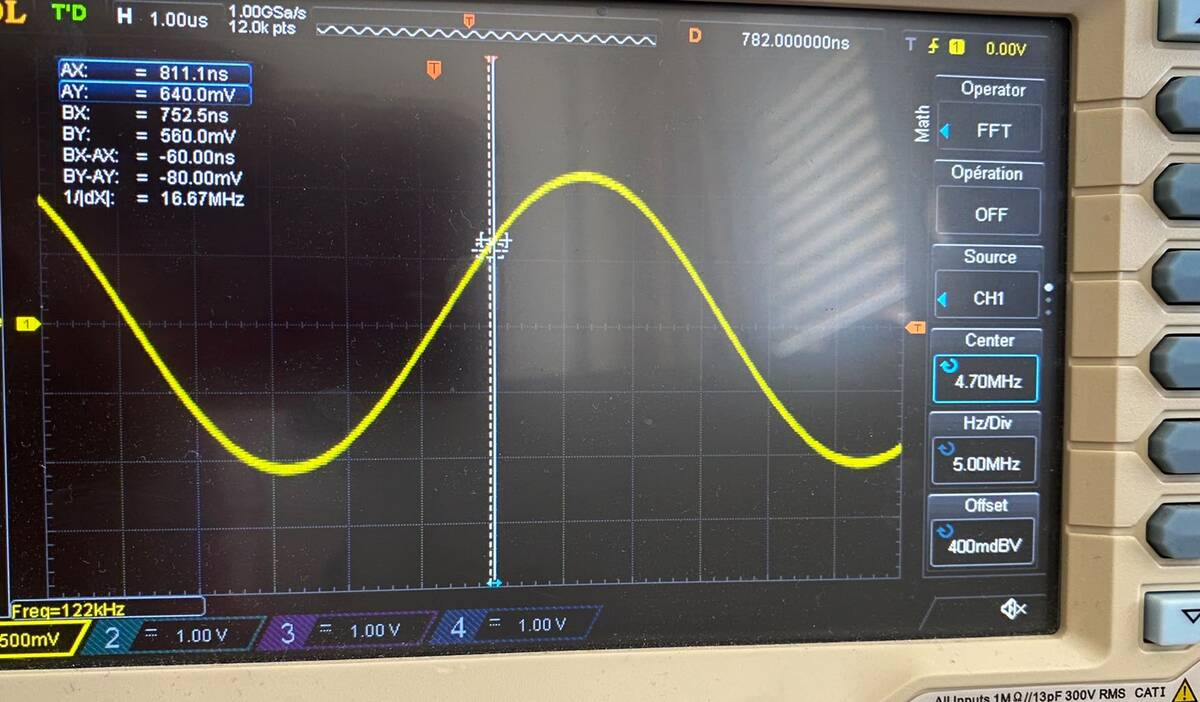
\includegraphics[width=\linewidth]{oscillo_W1.jpg}
  \caption{$W = 1$: \SI{122}{\kilo\hertz}, \SI{1}{\micro\second}/div}\label{fig:oscW1}
\end{subfigure}\hfill
\begin{subfigure}{0.49\linewidth}\centering
  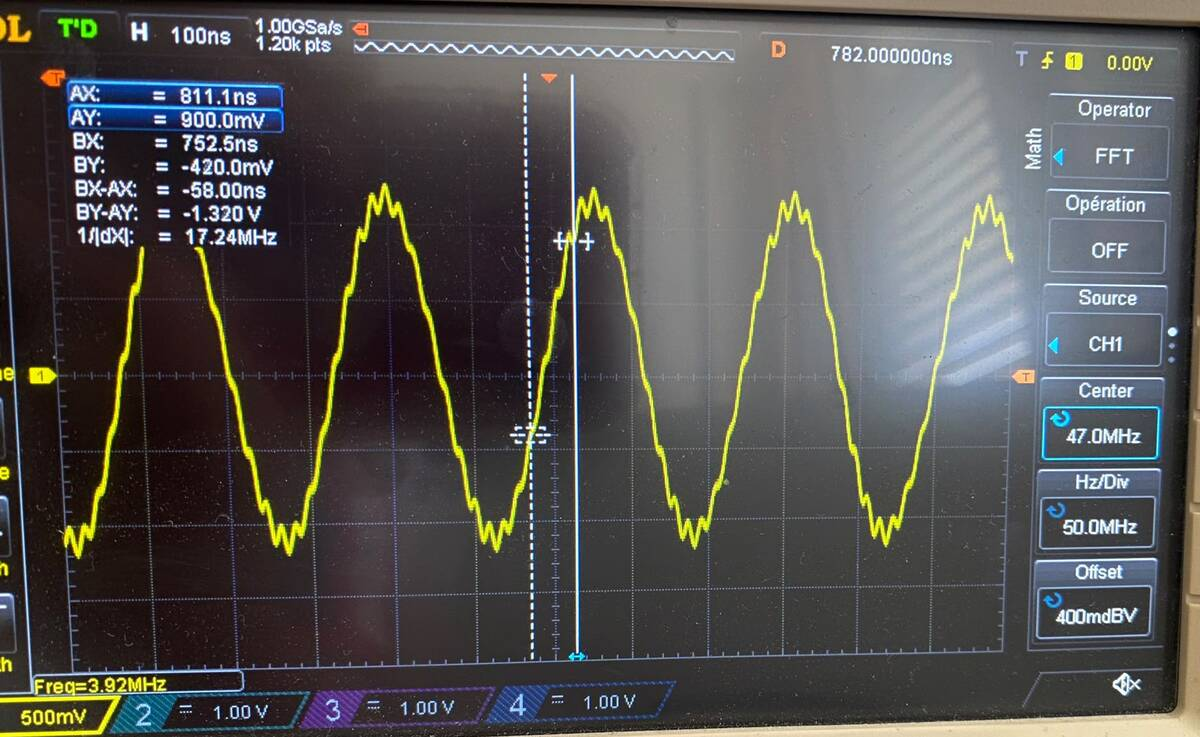
\includegraphics[width=\linewidth]{oscillo_W32.jpg}
  \caption{$W = 32$: \SI{3.92}{\mega\hertz}, \SI{100}{\nano\second}/div}\label{fig:oscW32}
\end{subfigure}

\medskip
\begin{subfigure}{0.49\linewidth}\centering
  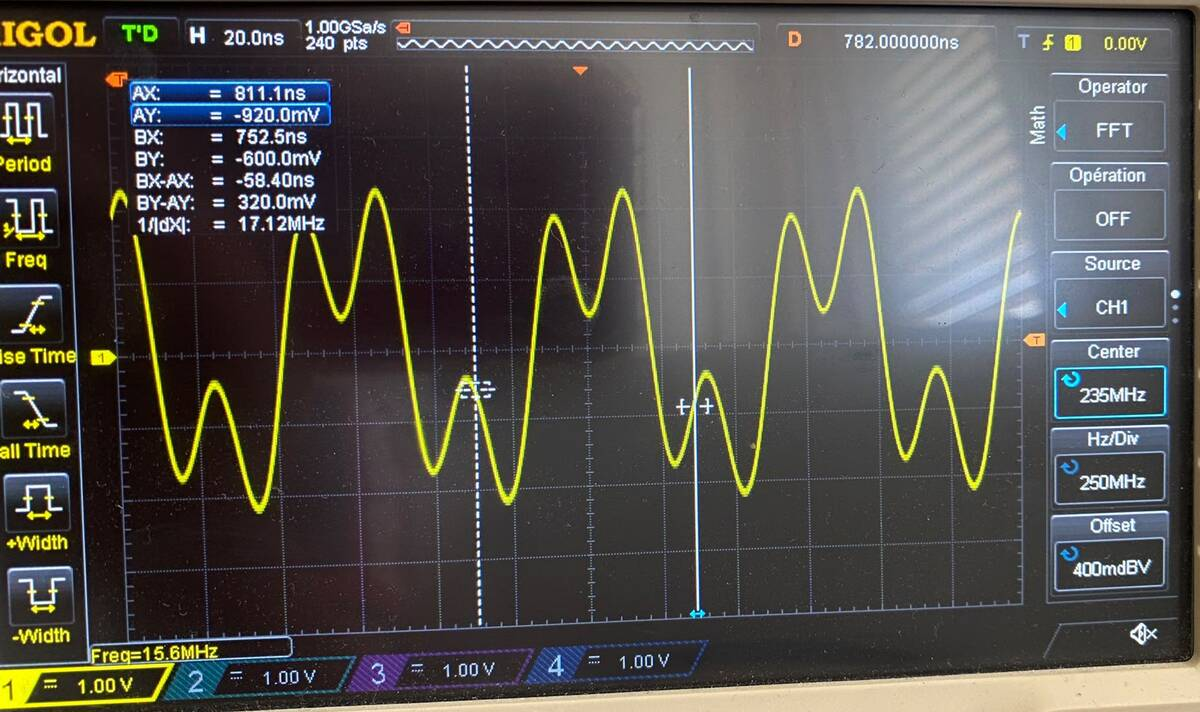
\includegraphics[width=\linewidth]{oscillo_W128.jpg}
  \caption{$W = 128$: \SI{15.6}{\mega\hertz}, \SI{20}{\nano\second}/div}\label{fig:oscW128}
\end{subfigure}
\caption{DAC output observed on the oscilloscope for three values of $W$}\label{fig:osc1}
\end{figure}

Table~\ref{tab:oscillo} shows that the board follows the formula
$f_{out} = f_{clk} \cdot W / 2^N$ for the eight values of $W$ tested, from 1 to 128.
The largest deviation, \SI{0.57}{\percent} at $W = 8$, stays below \SI{1}{\percent},
within the precision of the oscilloscope, which estimates the frequency from the few
periods displayed on screen.

As $W$ increases, the sine wave loses definition. At $W = 1$, each period contains
1024 samples and the output looks smooth (Figure~\ref{fig:oscW1}). At $W = 32$, only
32 samples remain and the steps become visible (Figure~\ref{fig:oscW32}). At
$W = 128$, the sine is distorted (Figure~\ref{fig:oscW128}): the DDS computes eight
samples per period, but the DAC converts only four of them, as explained below. The
board reproduces what the simulation showed in Figure~\ref{fig:simW4} and what
section~4.4 predicted: the fewer samples per period, the further the output moves
from a clean sine.

The output reaches about \SI{2}{\volt} peak to peak, or \SI{\pm 1}{\volt}, which
matches the full scale of the DAC: codes 0 to 16383 span the \SI{\pm 1}{\volt} range.

Small ripples appear on the signal, mostly near the peaks and troughs
(Figure~\ref{fig:oscW32}). We measured every signal with a \SI{50}{\ohm} termination
on a BNC T, so these ripples do not come from reflections in the cable. Their spacing
is of the order of \SI{16}{\nano\second}: they are the steps of the DAC output, which
holds each sample for two clock periods, smoothed by the \SI{50}{\mega\hertz}
bandwidth of the DS1054Z.

\paragraph{The DAC converts one sample out of two.} On the Red Pitaya, the AD9767
works in interleaved mode, and its datasheet states: ``\emph{In the interleaved mode,
IQCLK is divided by 2 internally. [\dots] the DAC latches are only updated on every
other rising edge of IQCLK.}'' With the \SI{125}{\mega\hertz} clock of the example file
(\texttt{dac\_clk\_o <= not clk125}), OUT1 is only updated 62.5 million times per
second: the frequency stays correct, but the DAC drops every other DDS sample. The
Vivado DAC block avoids this with a \SI{250}{\mega\hertz} clock. We checked it with a
second encapsulating file (Appendix~\ref{app:pl250}): a PLL (\texttt{PLLE2\_ADV})
generates \SI{250}{\mega\hertz} for the DAC and \SI{125}{\mega\hertz} for the DDS, and
the design alternates the DDS sample (channel A, OUT1) and mid-scale (channel B,
OUT2). With this version, $W = 128$ gives a clean sine at \SI{15.6}{\mega\hertz}.

% =====================================================================
\section{Control from Linux: PS / PL interaction}\label{sec:psps}

\subsection{Vivado block design}
\fig{block_design.png}{Vivado block design}{fig:bd}
Figure~\ref{fig:bd} shows the Vivado block design. Linux writes two 10-bit values
into the PL, and the PL turns them into a sine wave on OUT1. We follow the signal in
three passes: control, clocks, then data.

\paragraph{Control: from Linux to the DDS.} The Zynq PS runs Linux on the ARM cores
and reaches the PL through its master port \texttt{M\_AXI\_GP0}. The AXI Interconnect
(\texttt{ps7\_0\_axi\_periph}) routes these accesses to \texttt{axi\_gpio\_0}, mapped at
\texttt{0x4120\_0000}. \texttt{FCLK\_CLK0} clocks the AXI side, and
\texttt{proc\_sys\_reset\_0} generates the resets for the interconnect and the GPIO.
We configured the AXI GPIO with two output channels of 10 bits:
\begin{itemize}
  \item channel 1 (\texttt{gpio\_io\_o[9:0]}) drives \texttt{W[9:0]}, the phase
        increment that sets the DDS output frequency;
  \item channel 2 (\texttt{gpio2\_io\_o[9:0]}) drives \texttt{phase\_offset[9:0]},
        which shifts the phase of the sine.
\end{itemize}

\paragraph{Clocks.} The ADC board supplies a \SI{125}{\mega\hertz} differential clock on
\texttt{adc\_clk\_p/n}. \texttt{axis\_red\_pitaya\_adc\_0} outputs it as
\texttt{adc\_clk}, and \texttt{clk\_wiz\_0} derives two clocks from it:
\begin{itemize}
  \item \texttt{clk\_out1} at \SI{125}{\mega\hertz} for the DDS and the DAC interface
        (\texttt{aclk});
  \item \texttt{clk\_out2} at \SI{250}{\mega\hertz} for the DAC \texttt{ddr\_clk}
        input, which generates the \texttt{dac\_clk\_o} and \texttt{dac\_wrt\_o}
        signals of the converter.
\end{itemize}
The data leaves through DDR output registers clocked by \texttt{aclk}: they send
channel A on one clock edge and channel B on the other, which interleaves both
channels on the AD9767 bus. The DAC block also reads \texttt{locked} from the Clocking
Wizard: until both clocks settle, it holds its data at zero and keeps the converter
in reset.

\paragraph{Data: from the DDS to OUT1.} On each \texttt{clk\_out1} edge,
\texttt{dds\_0} outputs a 14-bit sample on \texttt{sine\_out[13:0]}.
The input \texttt{s\_axis\_tdata} of \texttt{axis\_red\_pitaya\_dac\_0} needs 32 bits,
so we fill the most significant bits with zeros, as the subject suggests:
\texttt{xlconcat\_0} places the sample on \texttt{In0[13:0]} and appends 18 zero bits
from \texttt{xlconstant\_1} on \texttt{In1[17:0]}. The DAC block reads channel A (OUT1)
from bits 13 to 0 of this word and channel B (OUT2) from bits 29 to 16. OUT1 carries
the sine; OUT2 receives zeros and stays at about \SI{0}{\volt}. \texttt{xlconstant\_0}
drives \texttt{s\_axis\_tvalid} with a constant 1, so the DAC accepts a sample on
every clock cycle without a handshake. We created this constant with a width of 14
bits and a value of 1; Vivado connects only its bit 0, equal to 1, to the 1-bit
\texttt{s\_axis\_tvalid} input and ignores the 13 others. A 1-bit constant would
avoid this width mismatch. The block then drives
\texttt{dac\_dat\_o[13:0]}, \texttt{dac\_clk\_o}, \texttt{dac\_rst\_o},
\texttt{dac\_sel\_o} and \texttt{dac\_wrt\_o} to the converter. The
\texttt{util\_ds\_buf} blocks on the daisy-chain connectors, \texttt{led\_o} and
\texttt{adc\_csn\_o} play no part in signal generation.

\paragraph{Role of the design.} Linux handles configuration and the PL handles
timing. A write of $W$ or the offset from user space lands in the GPIO registers
within a few bus cycles, and the DDS applies the new value on its next clock edge.
The processor never touches individual samples: the PL produces 125 million of them
per second on its own.

The GPIO outputs live in the \texttt{FCLK\_CLK0} domain while the DDS runs on
\texttt{clk\_out1}, derived from the ADC clock, and the design includes no
synchroniser between these two asynchronous domains. When $W$ or the offset changes,
the DDS may capture a mix of old and new bits during one clock cycle. A wrong offset
affects a single sample; a wrong $W$ adds one wrong phase step, which shifts the phase
of the sine for good but leaves its frequency unchanged. Since both values change
rarely, this is acceptable for this lab.

\subsection{Modification of \texttt{axis\_red\_pitaya\_dac.vhdl}}
The subject asks us to replace, in \texttt{axis\_red\_pitaya\_dac.vhdl},
\begin{lstlisting}[style=vhdl]
int_dat_a_reg <= int_dat_a_wire(DAC_DATA_WIDTH-1) & (not int_dat_a_wire(DAC_DATA_WIDTH-2 downto 0));
\end{lstlisting}
with
\begin{lstlisting}[style=vhdl]
int_dat_a_reg <= int_dat_a_wire(DAC_DATA_WIDTH-1 downto 0);
\end{lstlisting}

The original line converts a signed sample into the code the DAC expects; our DDS
already delivers that code, so the conversion must go.

\paragraph{Original line.} In the source project, \texttt{axis\_red\_pitaya\_dac}
receives the stream of \texttt{axis\_red\_pitaya\_adc}, which carries signed two's
complement samples. The original line keeps the most significant bit and inverts the
13 others, which turns a signed sample $x$ into the unsigned code $8191 - x$. The
AD9767 needs such an unsigned code: all 0s give \SI{0}{\milli\ampere} and all 1s the
full-scale current, and the Red Pitaya maps codes 0 to 16383 onto the
$\pm\SI{1}{\volt}$ output range.

\paragraph{Our DDS.} The DDS outputs an unsigned code $u$ from 0 to 16383, centred on
8192. This code already covers the $\pm\SI{1}{\volt}$ range: 0 and 16383 reach the
two ends and 8192 gives about \SI{0}{\volt}. The modified line passes $u$ to the DAC
unchanged.

\paragraph{Effect of the original line on our sine.} Keeping the MSB of $u$ and
inverting the other bits gives
\begin{equation}
  u' =
  \begin{cases}
    8191 - u  & \text{if } u < 8192,\\
    24575 - u & \text{if } u \geq 8192.
  \end{cases}
\end{equation}
The positive half-period stays in the upper half of the range but turns upside down,
the negative half-period does the same in the lower half, and the output jumps by
half the full scale each time the sine crosses 8192.

\paragraph{Check on the board.} Our first bitstream reused a DAC block that Vivado
had synthesised from the unmodified source project. Its synthesis report listed 26
\texttt{LUT1} inverters, 13 per channel, and with $W = 1$ OUT1 showed the mirrored
half-periods and jumps of Figure~\ref{fig:dacbefore}. After we refreshed the module
and synthesised it again, the report listed 13 \texttt{LUT1}, for channel B only, and
OUT1 gave a clean sine at \SI{122.1}{\kilo\hertz} (Figure~\ref{fig:dacafter}).

\begin{figure}[H]
\centering
\begin{subfigure}{0.49\linewidth}\centering
  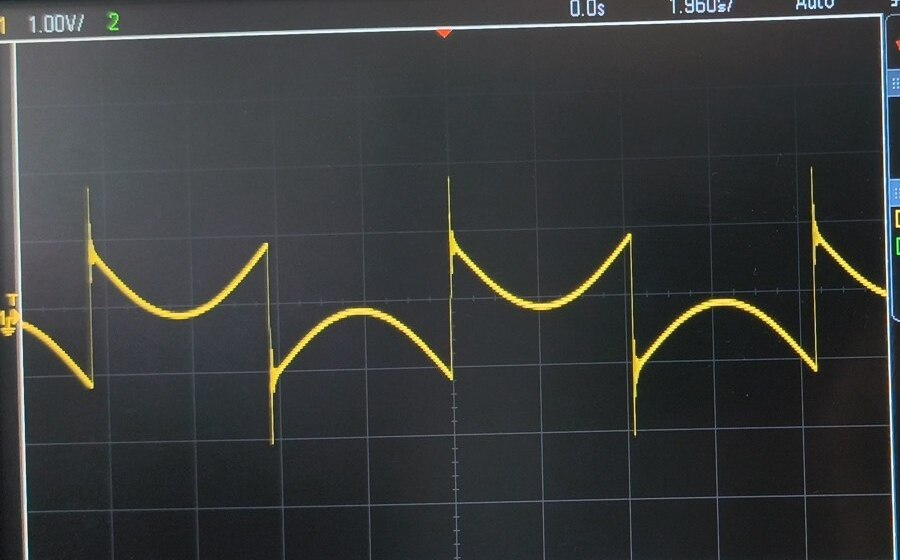
\includegraphics[width=\linewidth]{vivado_before_dac_fix.jpg}
  \caption{Original line (26 \texttt{LUT1})}\label{fig:dacbefore}
\end{subfigure}\hfill
\begin{subfigure}{0.49\linewidth}\centering
  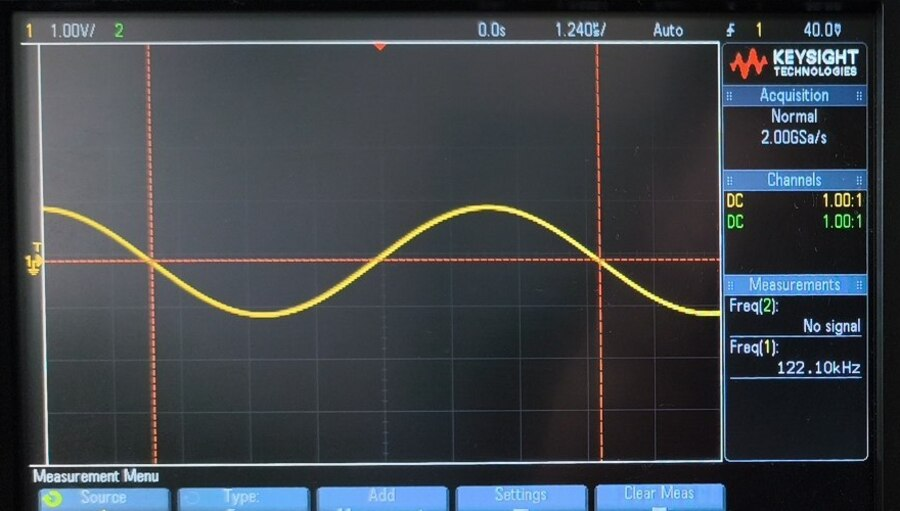
\includegraphics[width=\linewidth]{vivado_crop_w1.jpg}
  \caption{Modified line (13 \texttt{LUT1})}\label{fig:dacafter}
\end{subfigure}
\caption{DAC output on OUT1 for $W = 1$, before and after the modification of
\texttt{axis\_red\_pitaya\_dac.vhdl}}\label{fig:dacfix}
\end{figure}

\subsection{Programming from the Red Pitaya}
\begin{lstlisting}[style=sh, caption={Creating the .bit.bin and loading it}]
bootgen -image file.bif -arch zynq -process_bitstream bin
scp design_1_wrapper.bit.bin root@192.168.2.200:/tmp
# on the Red Pitaya:
cp /tmp/design_1_wrapper.bit.bin /lib/firmware/
echo design_1_wrapper.bit.bin > /sys/class/fpga_manager/fpga0/firmware
\end{lstlisting}

\subsection{Writing the registers with \texttt{devmem}}
\todo{registers used, values written, observations}

\begin{table}[H]
\centering
\begin{tabular}{rcccc}
\toprule
$W$ & Expected $f_{out}$ & Measured $f_{out}$ & Error & Measured Pk-Pk \\
\midrule
1    & \SI{122.07}{\kilo\hertz} & \SI{122.10}{\kilo\hertz} & \SI{+0.02}{\percent} & -- \\
2    & \SI{244.14}{\kilo\hertz} & \SI{244.23}{\kilo\hertz} & \SI{+0.04}{\percent} & -- \\
4    & \SI{488.28}{\kilo\hertz} & \SI{488.8}{\kilo\hertz}  & \SI{+0.11}{\percent} & -- \\
8    & \SI{976.56}{\kilo\hertz} & \SI{975.1}{\kilo\hertz}  & \SI{-0.15}{\percent} & -- \\
16   & \SI{1.953}{\mega\hertz}  & \SI{1.947}{\mega\hertz}  & \SI{-0.31}{\percent} & -- \\
64   & \SI{7.813}{\mega\hertz}  & \SI{7.81}{\mega\hertz}   & \SI{-0.03}{\percent} & -- \\
128  & \SI{15.625}{\mega\hertz} & \SI{15.6}{\mega\hertz}   & \SI{-0.16}{\percent} & \SI{3.02}{\volt} \\
256  & \SI{31.25}{\mega\hertz}  & \SI{31.3}{\mega\hertz}   & \SI{+0.16}{\percent} & \SI{2.09}{\volt} \\
512  & \SI{62.5}{\mega\hertz}   & \SI{62.4}{\mega\hertz}   & \SI{-0.16}{\percent} & \SI{0.80}{\volt} \\
513  & \SI{62.38}{\mega\hertz} (alias) & \SI{62.4}{\mega\hertz} & \SI{+0.03}{\percent} & \SI{0.07}{\volt} \\
1023 & \SI{122.07}{\kilo\hertz} (alias) & \SI{122.07}{\kilo\hertz} & \SI{0.00}{\percent} & \SI{2.07}{\volt} \\
\bottomrule
\end{tabular}
\caption{Output frequency for $W$ written with \texttt{devmem} (offset 0, Keysight
MSO-X~2002A, \SI{50}{\ohm} termination). For $W > 512$, the expected value is the
aliased frequency $f_{clk}(2^N - W)/2^N$.}\label{tab:devmem}
\end{table}

\begin{figure}[H]
\centering
\begin{subfigure}{0.32\linewidth}\centering
  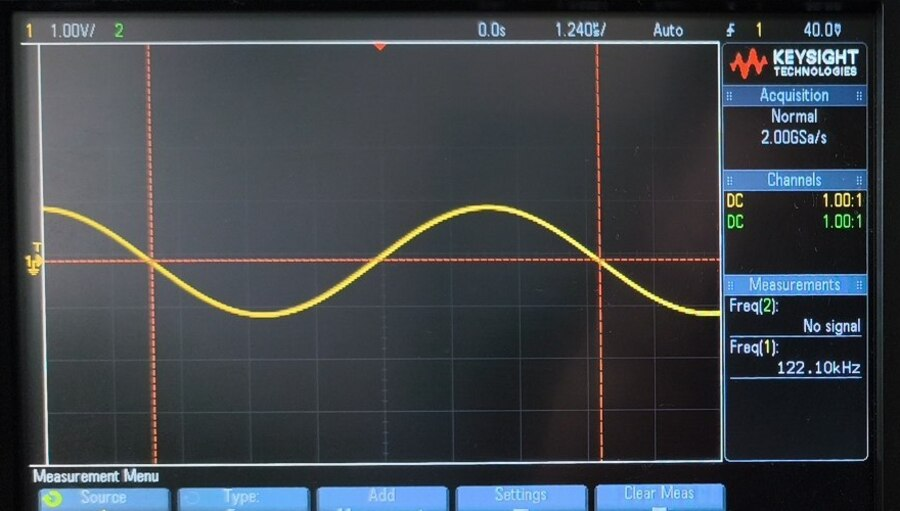
\includegraphics[width=\linewidth]{vivado_crop_w1.jpg}
  \caption{$W = 1$: \SI{122.10}{\kilo\hertz}}\label{fig:devW1}
\end{subfigure}\hfill
\begin{subfigure}{0.32\linewidth}\centering
  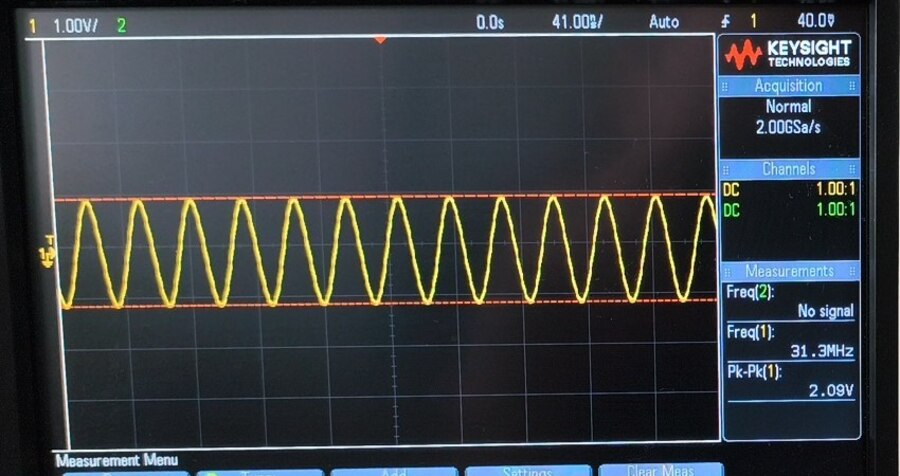
\includegraphics[width=\linewidth]{vivado_crop_w256.jpg}
  \caption{$W = 256$: \SI{31.3}{\mega\hertz}}\label{fig:devW256}
\end{subfigure}\hfill
\begin{subfigure}{0.32\linewidth}\centering
  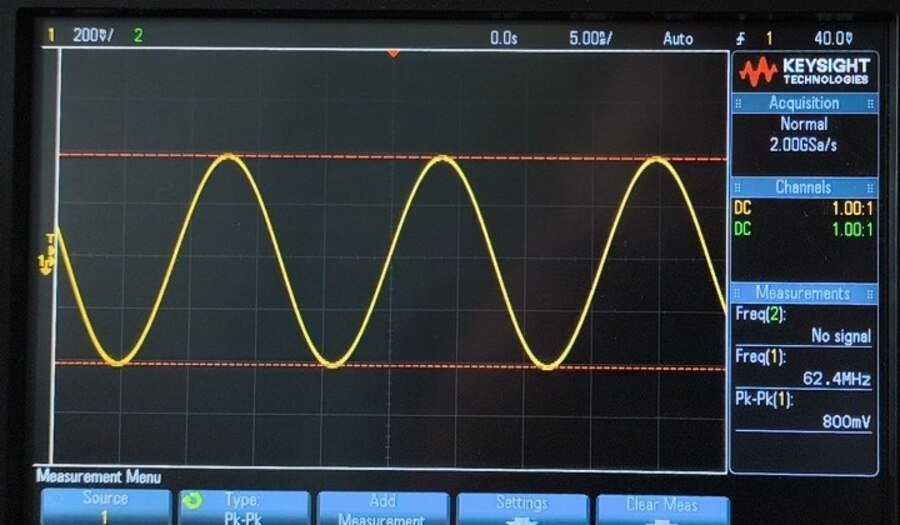
\includegraphics[width=\linewidth]{vivado_crop_w512.jpg}
  \caption{$W = 512$: \SI{62.4}{\mega\hertz}}\label{fig:devW512}
\end{subfigure}

\medskip
\begin{subfigure}{0.32\linewidth}\centering
  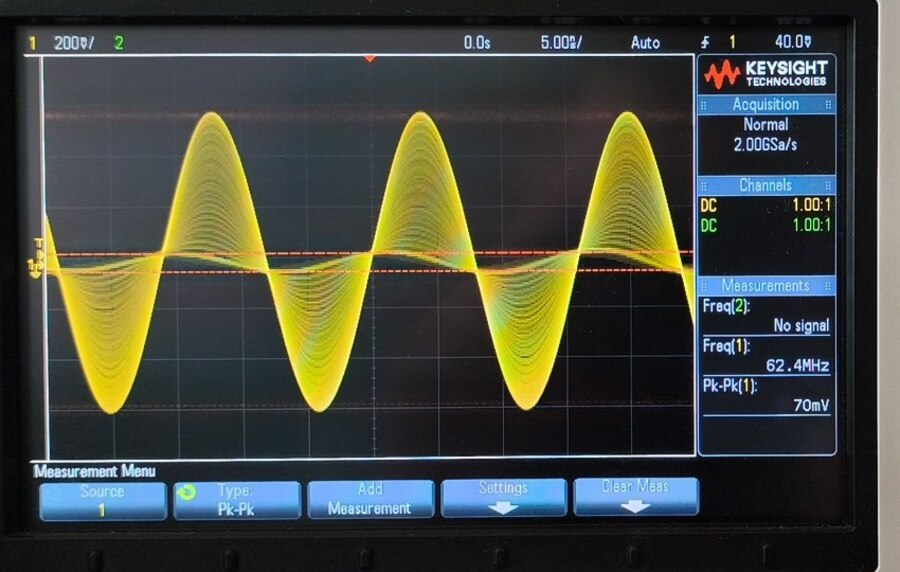
\includegraphics[width=\linewidth]{vivado_crop_w513.jpg}
  \caption{$W = 513$: \SI{62.4}{\mega\hertz}, varying amplitude}\label{fig:devW513}
\end{subfigure}\hspace{0.02\linewidth}
\begin{subfigure}{0.32\linewidth}\centering
  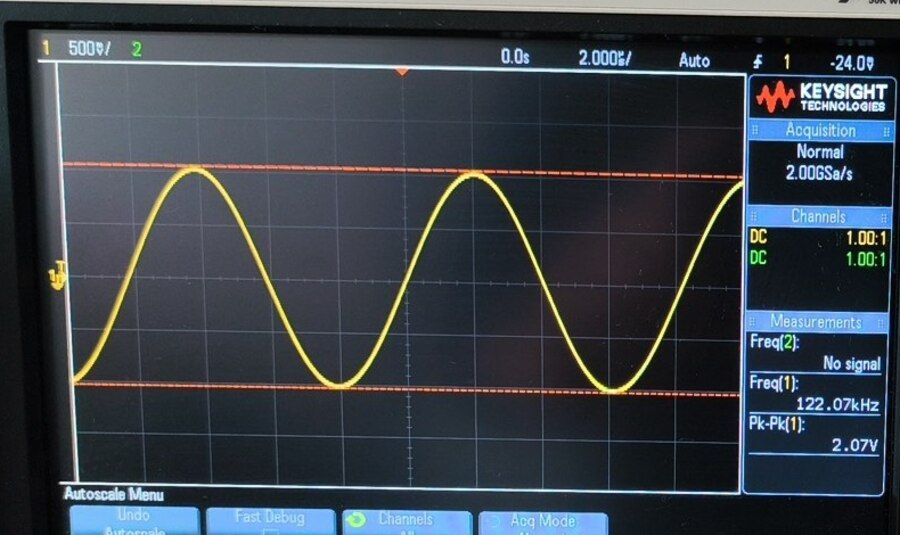
\includegraphics[width=\linewidth]{vivado_crop_w1023.jpg}
  \caption{$W = 1023$: \SI{122.07}{\kilo\hertz}}\label{fig:devW1023}
\end{subfigure}
\caption{DAC output (OUT1) for values of $W$ written from Linux with \texttt{devmem}}\label{fig:osc2}
\end{figure}

% =====================================================================
\section{Conclusion}
\todo{summary and what we learned}

% =====================================================================
\newpage
\appendix
\section{VHDL code}

\subsection{\texttt{dds.vhd}}
\lstinputlisting[style=vhdl]{../PL/dds.vhd}

\subsection{\texttt{dds\_tb.vhd}}
\lstinputlisting[style=vhdl]{../PL/dds_tb.vhd}

\subsection{\texttt{dds\_top.vhd}}
\lstinputlisting[style=vhdl]{../PL/dds_top.vhd}

\subsection{\texttt{dds\_top.vhd} with a \SI{250}{\mega\hertz} DAC clock}\label{app:pl250}
\lstinputlisting[style=vhdl]{../PL_250/dds_top.vhd}

\end{document}
